% !TEX root = sum1.tex
\section{Computational Experiment}\label{sec_result}
We carried out several experiments, including analyzing the performances of different policies, evaluating the impact of implementing social distancing, comparing different layouts, group sizes and social distancing. In the experiment, we set the following parameters. 

The default setting in the experiments is as follows, $\delta =1$ and $M =4$. The default seat layout consists of 10 rows, each with the same size of 21. The values of $\delta$, $M$ and the layout will change accordingly as we explore different layouts, group sizes and social distances.
We simulate the arrival of exactly one group in each period, i.e., $p_0 = 0$. The average number of individuals per period, denoted as $\gamma$, can be expressed as $\gamma = p_1 \cdot 1 + p_2 \cdot 2 + p_3 \cdot 3 + p_4 \cdot 4$, where $p_1$, $p_2$, $p_3$, and $p_4$ represent the probabilities of groups with one, two, three, and four individuals, respectively. We assume that $p_4$ always has a positive value.

\subsection{Performances of Different Policies}
In this section, we compare the performance of five assignment policies to the optimal one, which can be obtained by solving the deterministic model after observing all arrivals. The policies under examination are the dynamic seat assignment policy, DP-based heuristic, bid-price control, booking limit control and FCFS policy.

% [0.18, 0.7, 0.06, 0.06], [0, 0.5, 0, 0.5], [0.2, 0.8, 0 , 0]

% These distributions share the same value of $\gamma = 2.5$, ensuring that the expected number of individuals for each period remains consistent.

\subsection*{Parameters Description}
We consider three sets of probability distributions: D1: [0.18, 0.7, 0.06, 0.06], D2: [0, 0.5, 0, 0.5], D3: [0.2, 0.8, 0, 0], which are experimented in \cite{blom2022filling}. We also consider another probability distribution D4: [0.25, 0.3, 0.25, 0.2] for the extra experiments. The number of scenarios is $|\Omega| = 1000$. To assess the effectiveness of different policies across varying demand levels, we conducted experiments spanning a range of 60 to 100 periods. 


% By conducting experiments across this range of periods, we can observe how the different policies perform under both moderate and high-demand situations.

% For the DP Base-heuristic, we consider a simplified dynamic programming by relaxing all rows to a single row with the same total capacity, $\sum_{j=1}^{N} L_j$. With this simplification, we can make decisions for each group arrival based on the relaxed dynamic programming. 

% Bid-price control is a classical approach discussed extensively in the literature on network revenue management. It involves setting bid prices for different group types, which determine the eligibility of groups to take the seats. Specifically, we estimate the bid price of a seat by the shadow price of the capacity constraint in the LP relaxation of problem \eqref{deter_upper}. Then we assign the seats by comparing the revenues of accepting or denying the groups. 

% Booking limit control policy involves setting a maximum number of reservations for each group type. In this policy, we solve problem \eqref{deter_upper} with the expected demand during the time period. Then for every type of requests, we only allocate a fixed amount according to the static solution and reject all other exceeding requests.

The following table presents the performance results of five different policies: DSA, DP, Bid-price, Booking, and FCFS, which stand for dynamic seat assignment, dynamic programming based heuristic, bid-price, booking-limit, and first come first served, respectively. The procedures for the last four policies are detailed in the appendix \ref{policies}. Each entry in the table represents the average performance across 100 instances. Performance is evaluated by comparing the ratio of the number of accepted individuals under each policy to that under the optimal policy, which assumes complete knowledge of all incoming groups before making seat assignments.

\begin{table}[h]
  \centering
  \caption{Performances of Different Policies}
  \begin{tabular}{|c|c|c|c|c|c|c|}
  \hline
  Distribution & T & DSA (\%) & DP (\%) & Bid (\%) & Booking (\%) & FCFS (\%) \\
  \hline
  \multirow{5}{*}{D1} & 60 & 100.00 & 100.00 & 100.00 & 88.56 & 100.00 \\
  & 70    & 99.53 & 99.01 & 98.98 & 92.69 & 98.82 \\
  & 80    & 99.38 & 98.91 & 98.84 & 97.06 & 96.06 \\
  & 90    & 99.52 & 99.23 & 99.10 & 98.24 & 95.37 \\
  & 100   & 99.58 & 99.27 & 98.95 & 98.46 & 94.98 \\
  \hline
  \multirow{5}{*}{D2} & 60  & 99.45 & 97.23 & 96.58 & 99.09 & 96.49 \\
     & 70   & 99.82 & 98.28 & 97.46 & 99.81 & 95.76 \\
     & 80   & 99.92 & 98.60 & 98.86 & 100.00 & 95.66 \\
     & 90   & 99.99 & 99.10 & 99.70 & 100.00 & 95.66 \\
     & 100  & 100.00 & 98.74 & 99.99 & 100.00 & 95.66 \\
  \hline
  \multirow{5}{*}{D3} & 60  & 100.00 & 100.00 & 100.00 & 93.68 & 100.00 \\
     & 70  & 100.00 & 100.00 & 100.00 & 92.88 & 100.00 \\
     & 80  & 99.54 & 97.89 & 97.21 & 98.98 & 96.19 \\
     & 90  & 99.90 & 99.73 & 99.44 & 99.61 & 94.53 \\
     & 100 & 100.00 & 100.00 & 100.00 & 99.89 & 94.32 \\
  \hline
    \multirow{5}{*}{D4} & 60  & 99.61 & 99.68 & 99.63 & 94.01 & 99.61 \\
     & 70  & 99.05 & 98.95 & 98.49 & 97.10 & 96.03 \\
     & 80  & 98.96 & 98.84 & 98.71 & 97.99 & 93.80 \\
     & 90  & 99.38 & 99.17 & 98.70 & 98.36 & 92.87 \\
     & 100 & 99.62 & 99.45 & 99.13 & 98.56 & 92.35 \\
  \hline
  \end{tabular}
\end{table}

We can find that DSA is better than DP-based heuristic, bid-price policy and booking limit policy consistently, and FCFS policy works worst. DP-based heuristic and bid-price policy can only make the decision to accept or deny, cannot decide which row to assign the group to. Booking limit policy does not consider using more seats to meet the demand of one group. FCFS accepts groups in sequential order until the capacity cannot accommodate more.

The performance of DSA, DP-based heuristic, and bid-price policies follows a pattern where it initially decreases and then gradually improves as $T$ increases. When $T$ is small, the demand for capacity is generally low, allowing these policies to achieve relatively optimal performance. However, as $T$ increases, it becomes more challenging for these policies to consistently achieve a perfect allocation plan, resulting in a decrease in performance. Nevertheless, as $T$ continues to grow, these policies tend to accept larger groups, thereby narrowing the gap between their performance and the optimal value. Consequently, their performances improve. In contrast, the booking limit policy shows improved performance as $T$ increases because it reduces the number of unoccupied seats reserved for the largest groups. 

% When $T$ increases to infinity, DSA can always generate the largest pattern in each row, thus, the performance will converge to 100\% compared to the optimal solution.

The performance of the policies can vary based on different probabilities. For the different probability distributions listed, DSA performs more stably and consistently for the same demand. In contrast, the performance of DP and bid-price fluctuates more significantly.

% Moreover, according to the results of policies, we can develop an easy-to-implement policy. When $T \leq \frac{\sum_{j}{L_j}}{\gamma + 1}$, we accept the groups based on the first come first served policy. When $T > \frac{\sum_{j}{L_j}}{\gamma + 1}$, we adopt the booking-limit policy, i.e., assign the seats according to the seat planning obtained from problem \eqref{deter_upper}.

% \subsection*{Analysis of DSA}
% We explore the arrival path of one instance under DSA and the optimal solution. The figures show two arrival paths when $T= 55$ and $T= 70$ at the even probability distribution. In the figures, we plot four lines over periods, number of remaining seats, the expected future demand, optimal remaining seats and optimal remaining demand. The horizontal parts of remaining seats represent the rejection at the period. We can observe that when the demand is larger than supply (T =70), even at the beginning we still reject the group. When the demand is lower than supply (T =55), we will accept all groups.


% We also examine the situations where the actual demand is higher or lower than the expected demand.

% Based on the figures provided, we can draw several key conclusions:

% 1. When the demand is larger than supply, even at the very beginning of the time period, both DSA approach and the optimal solution reject some groups, as indicated by the horizontal segments in the lines.

% 2. DSA approach is inclined to accept groups earlier compared to the optimal solution. This is because DSA makes decisions based on the expected future demand, rather than the actual remaining demand.

% 3. When the actual remaining demand is lower than the expected demand, the optimal remaining seats will be lower than that of DSA approach. Conversely, when the actual remaining demand is higher than expected, the optimal remaining seats will be higher than DSA.

% For the DSA, DP Base-heuristic, bid-price policies, their performance tends to initially drop and then increase as the number of periods increases. When the number of periods is small, the demand for capacity is relatively low, and the policies can achieve relatively optimal performance. However, as the number of periods increases, the policies may struggle to always obtain a perfect allocation plan, leading to a decrease in performance. Nevertheless, when the number of periods continue to become larger, these policies tend to accept larger groups, and as a result, narrow the gap with the optimal value, leading to an increase in performance. As the number of periods increases, the performance for the booking limit policy is getting better because the numebr of seats planned for the largest groups that are not occupied will drop.

\subsection{Impact of Social Distancing}
Now, we explore the impact of social distance as the demand increases. Specifically, we consider $D4$ as the probability distribution. In the next section, we also consider other distributions. Here, $T$ varies from 30 to 90, the step size is 1. Other parameters are set the same as before.

% It is evident that as the demand increases, the effect of social distancing becomes more pronounced. We aim to determine the specific time period where the absence of social distancing results in a higher number of accepted individuals compared to when social distancing measures are in place. Additionally, we will calculate the corresponding occupancy rate during this period.

% By analyzing and comparing the data, we can gain insights into the relation between demand, social distancing, the number of accepted individuals, and occupancy rates. This information is valuable for understanding the impact of social distancing policies on overall capacity utilization and making informed decisions regarding resource allocation and operational strategies.


The figure below displays the outcomes of groups who were accepted under two different conditions: with social distancing measures and without social distancing measures. For the former case, we employ DSA to obtain the results. In this case, we consider the constraints of social distancing and optimize the seat allocation accordingly. For the latter case, we adopt the optimal solution assuming that all arrivals are known and that there are no social distancing constraints. The occupancy rate at different demands is calculated as the average of these 100 instances. The figures depicting the results are presented below. The difference between these two figures is the x-axis, the left one is period, while the right one is the percentage of expected demand relative to total seats. 

% We simply accept all incoming groups if the capacity allows, without considering the constraints of social distancing. 

\begin{figure}[h]
  \centering
  \subfigure[]{
    \label{typical_figure}
    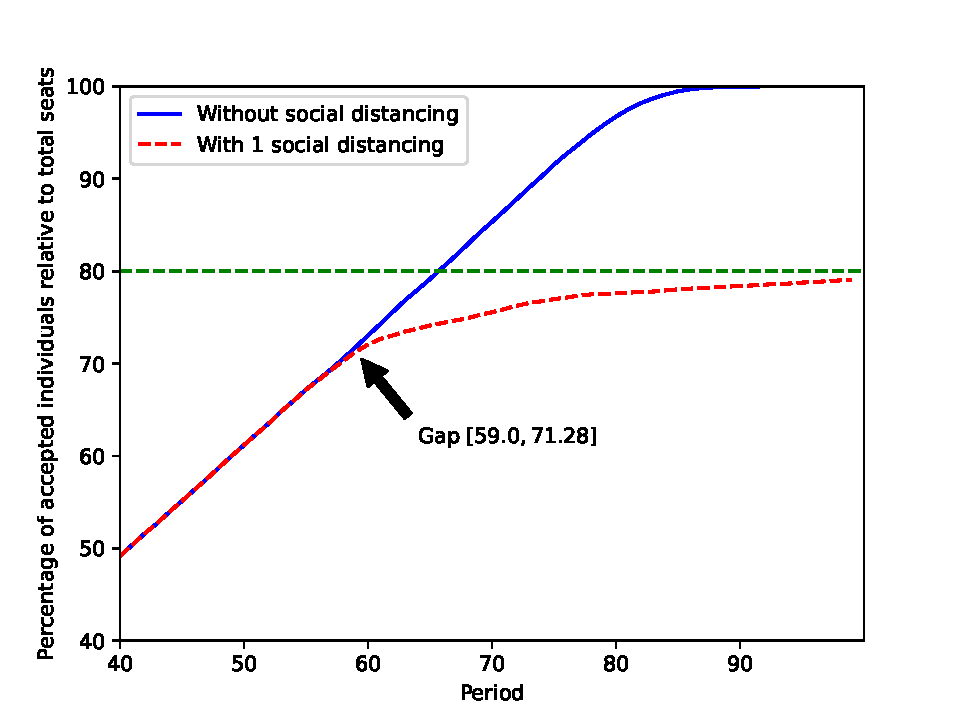
\includegraphics[width=0.48\textwidth]{./Figures/occu_demand_group4.pdf}}
  \subfigure[]{
    \label{Fig.sub.2}
    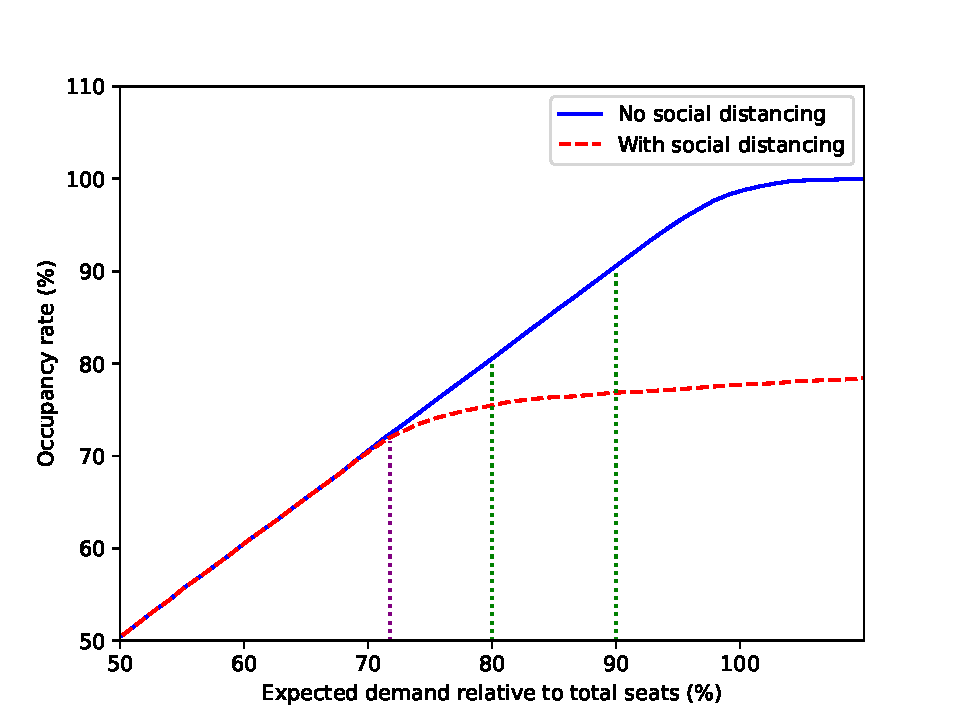
\includegraphics[width=0.48\textwidth]{./Figures/occu_gamma_group4.pdf}}
  \caption{The occupancy rate over demand}
  \label{Fig.lable}
\end{figure}

Intuitively, when demand is low, we will accept all arrivals, and there will be no difference in the number of accepted individuals whether we implement social distancing or not. The interesting case is when the difference in the number of accepted individuals due to social distancing starts to occur.

We use $E(T; DSA)$ to denote the expected number of individuals accepted across 100 instances by DSA with one seat as social distancing. Similarly, we use $E(T; OPT)$ to denote the expected number of individuals accepted across 100 instances by the optimal solution when there is no social distancing. The gap point $\tilde{T}$ is defined as the largest point $T$ such that $E(T; DSA)+1 \geq E(T; OPT)$ holds. The occupancy rate at the gap point is denoted by $\Gamma(\tilde{T})$. This occupancy rate represents the maximum demand that can be satisfied when the difference in the number of accepted individuals is not affected by social distancing.

% 代表了当有社交距离的要求但不受社交距离影响能达到的最大需求
% This period marks the threshold where the difference in the number of accepted individuals due to social distancing becomes significant.

Under the probability distribution of $D4$, we obtain the gap point is 60, the corresponding occupancy rate is 71.8\%. To better analyze the situation under different demands, we plot the second figure. When the expected demand is less than 71.8\%, the social distancing measures will not have an impact. When the expected demand is larger than 71.8\%, the difference between the number of accepted individuals with and without social distancing measures becomes more pronounced. As the expected demand continues to increase, both situations reach their maximum capacity acceptance. At this point, the gap between the outcomes with and without social distancing measures begins to converge. For the social distancing situation, according to Proposition \ref{lem_pattern}, when the largest pattern is assigned to each row, the resulting occupancy rate is $\frac{16}{20} = 80\%$, which is the upper bound of occupancy rate. Therefore, the policy requires an occupancy rate larger than 80\% will be invalid.

% 由于 occupancy rate 已经被social distancing 所限定,因此政府额外设置occupancy rate 是不必要的

\subsection{Estimation of Gap Points}
To estimate the gap point, we aim to find the maximum period such that all the groups can be assigned into the seats during these periods, i.e., for each group type $i$, we have $\sum_{j} x_{ij} \geq d_i$, where $x_{ij}$ is the number of group type $i$ in row $j$. Meanwhile, we have the capacity constraint $\sum_{i} n_{i} x_{ij} \leq L_j$, thus, $\sum_{i} n_i d_i \leq \sum_{i} n_i \sum_{j} x_{ij} \leq \sum_{j} L_{j}$. Notice that $E(d_i) = p_i T$, we have $\sum_{i} n_i p_i T \leq \sum_{j} L_{j}$ by taking the expectation. Recall that $\tilde{L} = \sum_{j} L_{j}$ denotes the total number of seats, and let $\gamma = \sum_{i} i p_i$ represent the expected number of individuals arriving in each period. From this, we can derive the inequality $T \leq \frac{\tilde{L}}{\gamma + \delta}$. Therefore, the upper bound for the expected maximum period is given by $T' = \frac{\tilde{L}}{\gamma + \delta}$.


Assuming that we accept all incoming groups within $T'$ periods, filling all the available seats, the corresponding occupancy rate at this period can be calculated as $\frac{\gamma T'}{(\gamma+ \delta)T' - N \delta} = \frac{\gamma}{\gamma +\delta} \frac{\tilde{L}}{\tilde{L}-N \delta}$. However, it is important to note that the actual maximum period will be smaller than $T{'}$ because it is impossible to accept groups to fill all seats exactly. To estimate the gap point when applying DSA, we can use $y_1 = c_1 \frac{\tilde{L}}{\gamma + \delta}$, where $c_1$ is a discount factor compared to the ideal assumption. Similarly, we can estimate the corresponding occupancy rate as $y_2 = c_2 \frac{\gamma}{\gamma +\delta} \frac{\tilde{L}}{\tilde{L}-N \delta}$, where $c_2$ is a discount factor for the occupancy rate compared to the ideal scenario.

To analyze the relation between the increment of $\gamma$ and the gap point, we conducted an analysis using a sample of 200 probability distributions. The figure below illustrates the gap point as a function of the increment of $\gamma$, along with the corresponding estimations. For each probability combination, we considered 100 instances and plotted the gap point as blue points. Additionally, the occupancy rate at the gap point is represented by red points.

% we define each distribution $(p_1, p_2, p_3, p_4)$ satisfying $p_1 + p_2 + p_3 + p_4 = 1$ as a probability combination. 

To provide estimations, we use the equations $y_1 = \frac{c_1 \tilde{L}}{\gamma + \delta}$ (blue line in the figure) and $y_2 = c_2 \frac{\gamma}{\gamma + \delta} \frac{\tilde{L}}{\tilde{L}-N \delta}$ (orange line in the figure), which are fitted to the data. These equations capture the relationship between the gap point and the increment of $\gamma$, allowing us to approximate values. By analyzing this relationship, we find that $\gamma$ can be utilized to estimate the gap point. We employed an Ordinary Least Squares (OLS) model to fit the data and derive the parameter values. The goodness of fit is assessed using the R-squared values of 1.000 for all models, indicating a perfect fit between the data and the models. Here, the values of the discount factors are $c_1 = 0.9578$ and $c_2 = 0.9576$.

\begin{figure}[ht]
  \centering
    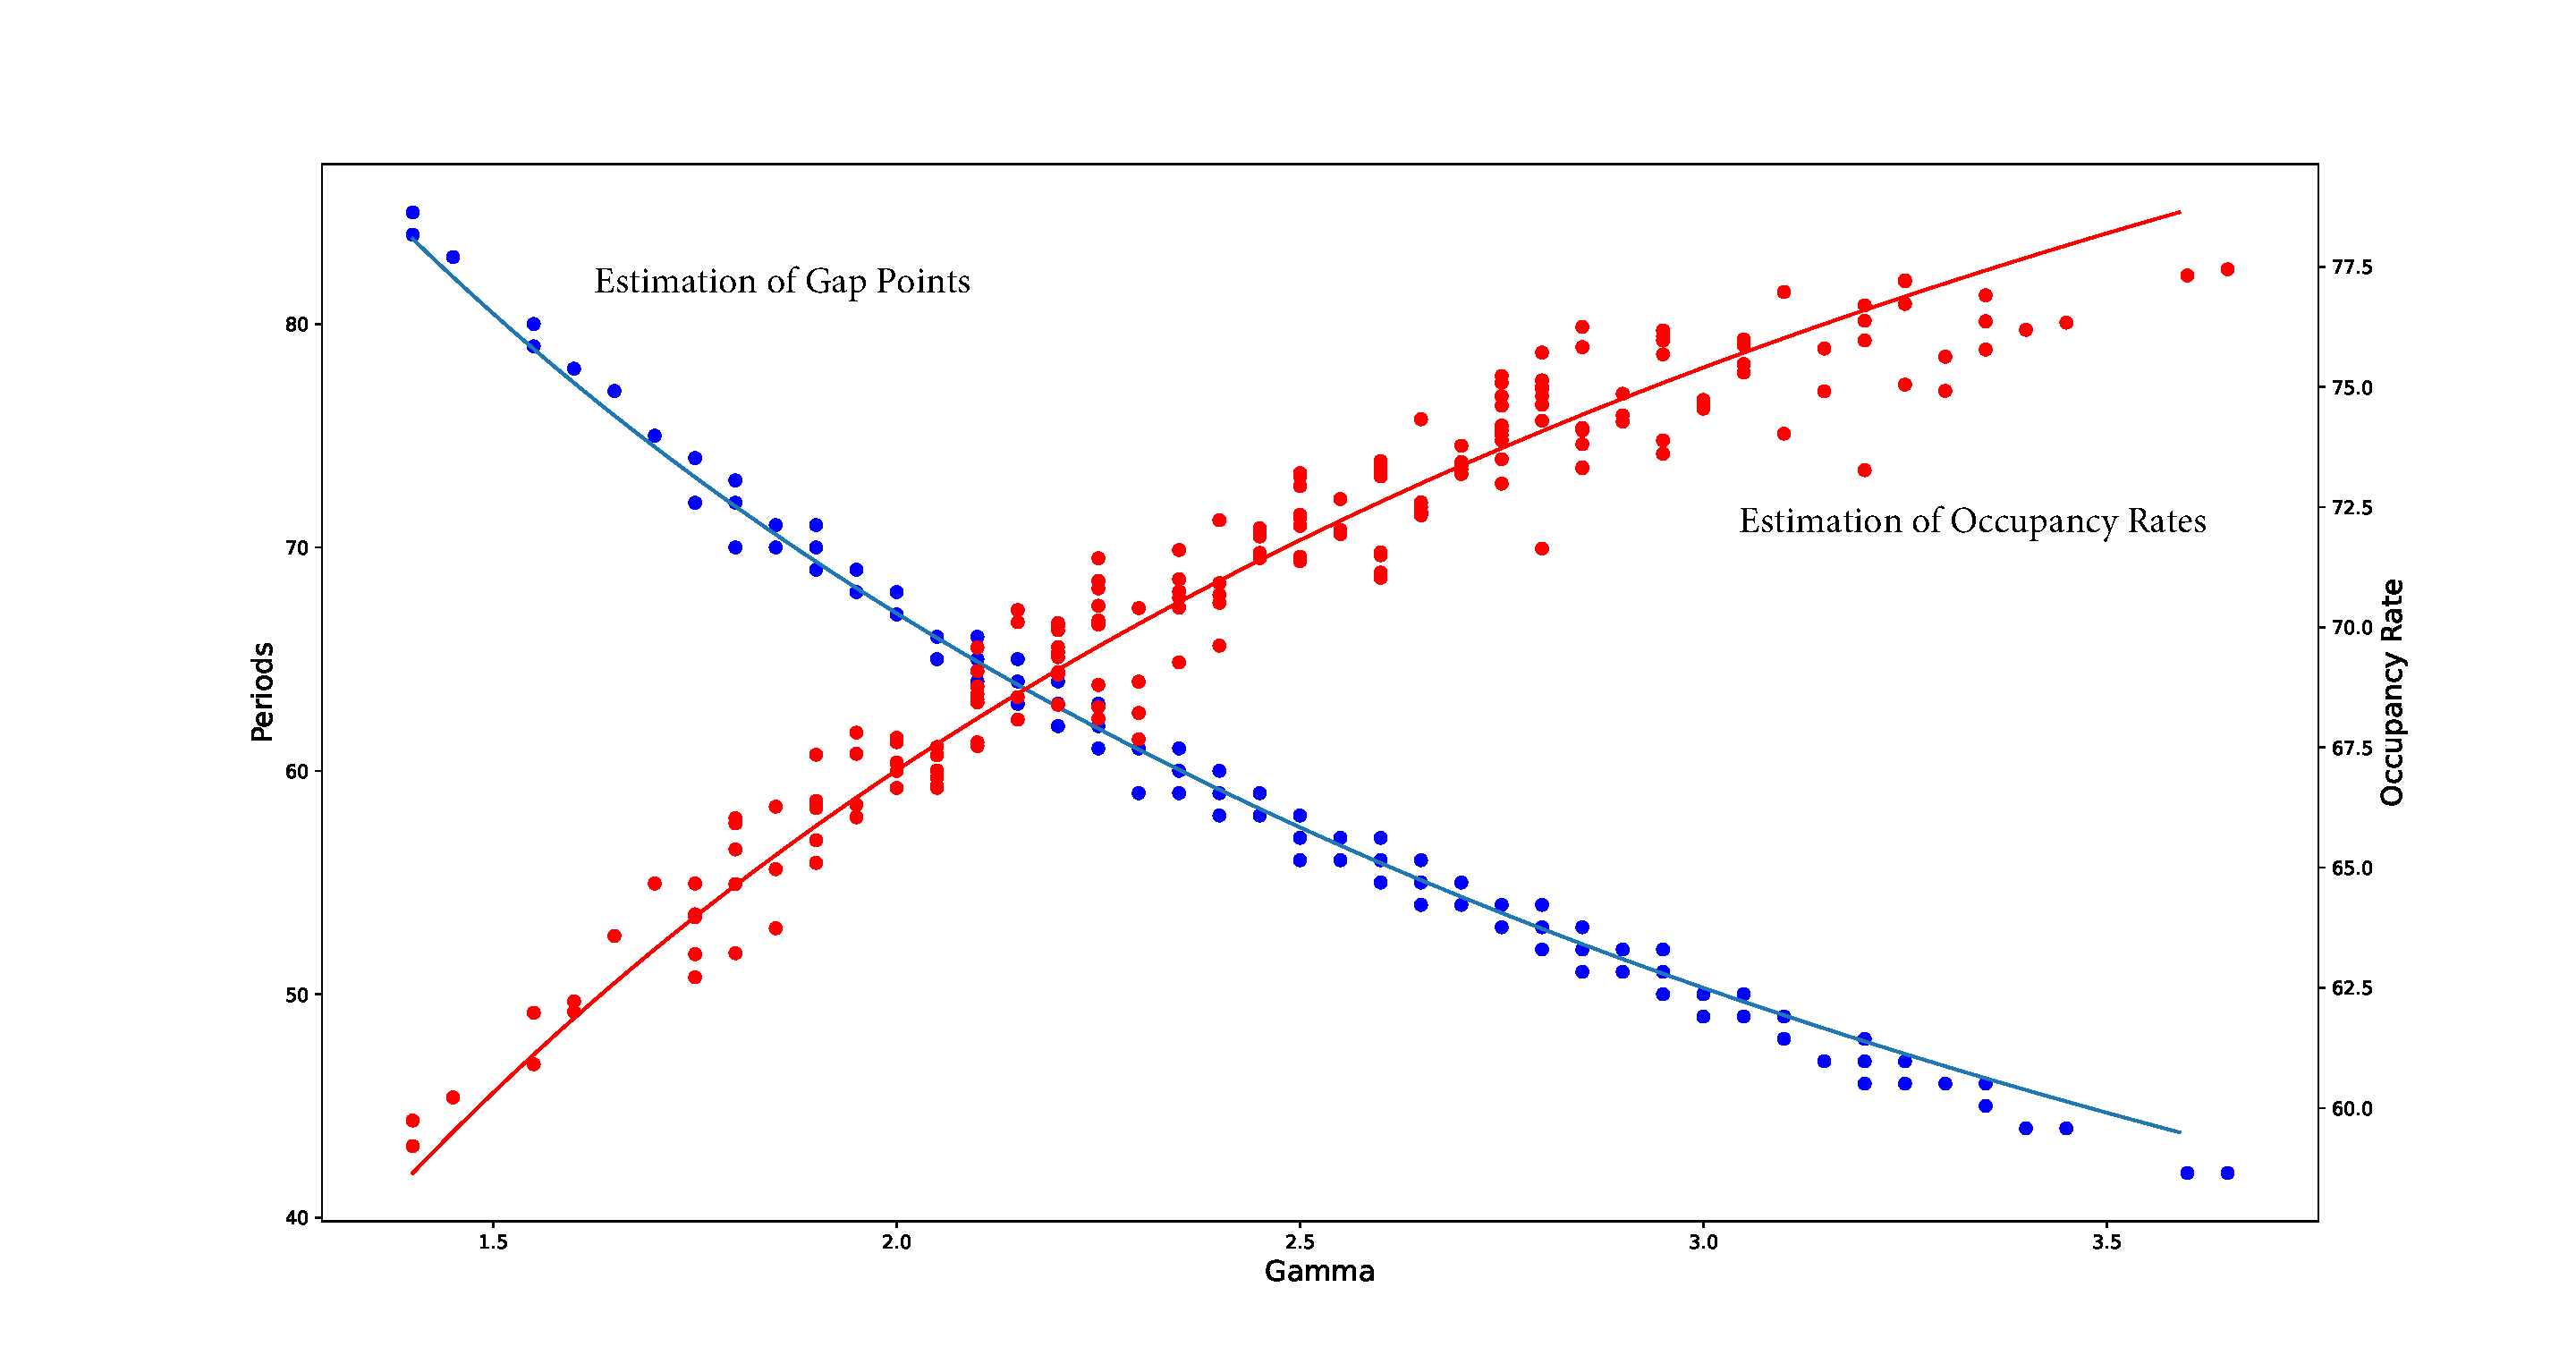
\includegraphics[width=0.95\textwidth]{./Figures/gamma_estimation.pdf}
  \caption{Gap points and their estimation under 200 probabilities}
\end{figure}

% The fitting values of $c_1$ and $c_2$ can be affected by different seat layouts. To investigate this impact, we conduct several experiments using different seat layouts, specifically with the number of rows $\times$ the number of seats configurations set as 10 $\times$ 16, 10 $\times$ 21, 10 $\times$ 26 and 10 $\times$ 31. Similarly, we perform an analysis using a sample of 100 probability combinations, each with a mean equal to $\gamma$. The values of $\gamma$ range from 1.5 to 3.4.

% The results of the estimation of $c_1$ and $c_2$ are presented in the table below:

% \begin{table}[ht]
%   \centering
%   \caption{Fitting values of $c_1$ and $c_2$}
%   \begin{tabular}{|c|c|c|}
%   \hline
%    Seat Layout & Fitting Values of $c_1$ & Fitting Values of $c_2$  \\
%   \hline
%    Layout 1 & 0.909 $\pm$ 0.013  & 89.89 $\pm$ 1.436 \\
%    Layout 2 & 0.948 $\pm$ 0.008  & 94.69 $\pm$ 0.802 \\
%    Layout 3 & 0.955 $\pm$ 0.004 & 95.44 $\pm$ 0.571 \\
%    Layout 4 & 0.966 $\pm$ 0.004 & 96.23 $\pm$ 0.386 \\
%    \hline
%   \end{tabular}
% \end{table}


% Since the gap points of different probability distributions with the same $\gamma$ show little variation, we use the following probability distributions for $\gamma$ values ranging from 1.9 to 2.7: [0.45, 0.35, 0.05, 0.15], [0.35, 0.35, 0.15, 0.15], [0.35, 0.25, 0.15, 0.25], [0.3, 0.2, 0.2, 0.3], [0.25, 0.15, 0.25, 0.35]. For each distribution, we simulate 100 instances to calculate the occupancy rate. 
% As the value of $\gamma$ increases, the gap point will decrease and the corresponding occupancy rate will increase. Consequently, the occupancy rate increases due to the allocation of seats to larger groups. The percentage difference is negligible when the demand is small, but it becomes more significant as the demand increases.

% This suggests that larger groups are more likely to be accepted, resulting in a smaller number of accepted groups overall. 

Based on the above analysis, we also explore the results of different layouts, different group sizes and different social distances. Since the figure about the occupancy rate over demand is similar to Figure \ref{typical_figure}, we only use three metrics to show the results: the gap point and the corresponding occupancy rate, largest occupancy rate.

\subsection*{Different Layouts}
We experiment with four seat layouts. For the large room, we consider three configurations, each with the same total of 200 seats. Layout 1 consists of 20 rows with 10 seats each, Layout 2 features 10 rows with 20 seats each. Additionally, we include a fan-shaped Layout 3 with 10 rows, where the first five rows contain between 16 and 20 seats, increasing by 1 seat per row, and the last five rows contain between 20 and 24 seats, also increasing by 1 seat per row. This ensures that the total number of seats and the number of rows match those of the Layout 2. Layout 4 as the small room consists of 15 rows with 7 seats each. The same 100 instances with the probability of $D4$ are experimented for each layout.

The occupancy rate over demand follows the typical pattern of Figure \ref{typical_figure}. The gap point, the corresponding occupancy rate and the largest occupancy rate are also given in the following table. The largest occupancy rate can be calculated from Proposition \ref{lem_pattern}.

% \begin{figure}[h]
%   \centering
%     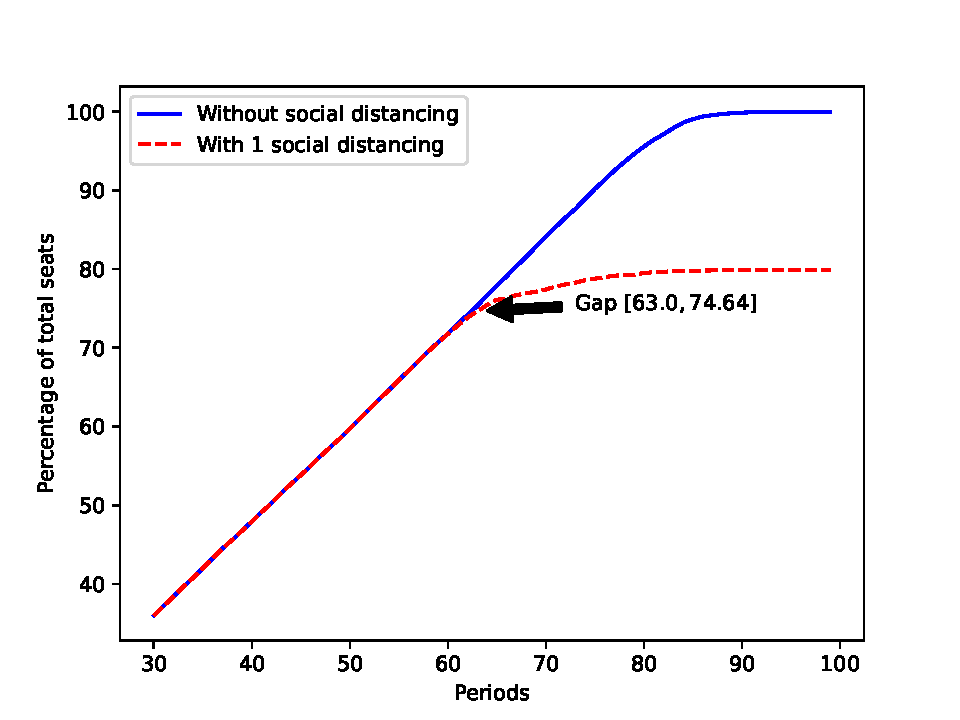
\includegraphics[width=0.8\textwidth]{./Figures/layout20.pdf}
%   \caption{The occupancy rate over demand with Layout 1}
% \end{figure}

\begin{table}[ht]
  \centering
  \caption{Gap points and occupancy rates of the layouts}
  \begin{tabular}{|c|c|c|c|}
  \hline
   Seat Layout & Gap point & Occupancy rate & Largest occupancy rate \\
  \hline
   Layout 1 & 62.0 & 74.33 \% & 80 \% \\
   Layout 2 & 60.0 & 71.79 \% & 80 \% \\ 
   Layout 3 & 60.0 & 71.84 \% & 82 \% \\
   Layout 4 & 33.0 & 74.41 \% & 85.71 \% \\
   $[4,6,8,10,10]$ & 12 & 72.18 \% &  \\
   14seats 11rows & 46 & 71.48 \% &  \\
   6seats 6 rows & 11 & 69.67 \% &  \\
   Large not rec & 75 & 72.88 \% &  \\
   \hline
  \end{tabular}
\end{table}

We have three observations. First, the gap point and occupancy rate of Layout 1 are higher than those of Layout 2 and Layout 3. This suggests that, when the total number of seats is the same, the layout with more rows yields a larger gap point and occupancy rate compared to the layout with fewer rows.
Second, when the number of rows is the same, the fan-shaped layout exhibits a similar gap point and occupancy rate to the rectangular layout. However, the largest occupancy rates differ between the two layouts. Third, the occupancy rate at the gap point and the largest occupancy rate for the small room will be higher than those for the large room, comparatively.

For each row, a seat is designated for social distancing with every group accepted. Consequently, when each row follows a full pattern and the total number of seats remains constant, having more rows results in a higher gap point and occupancy rate. Similarly, in a small room with fewer seats per row, the occupancy rate at the gap point will correspondingly be higher.


\subsection*{Different Group Sizes}
For group sizes of 3, 4 and 5, we present the gap point, the corresponding occupancy rate and the largest occupancy rate in the table below. The probability distributions for these group sizes all share the same value of $\gamma = 2.4$.

% The figures display the number of accepted individuals over time for group sizes of 3 and 5, respectively, both sharing the same average group of people.

\begin{table}[ht]
  \centering
  \caption{Gap points and occupancy rates of the group sizes}
  \begin{tabular}{|c|c|c|c|c|}
  \hline
   Group Size & Probability distribution & Gap point & Occupancy rate & Largest occupancy rate \\
  \hline
   3 & [0.2, 0.2, 0.6] & 60.0  & 71.83 \% & 75 \% \\
   4 & [0.25, 0.3, 0.25, 0.2] & 60.0 & 71.79 \% & 80 \%  \\ 
   5 & [0.3, 0.3, 0.2, 0.1, 0.1] & 58.0 & 70.00 \% & 85 \% \\
   \hline
  \end{tabular}
\end{table}

We observe that larger group sizes correspond to higher largest occupancy rates under the same seat layout. However, the gap point and occupancy rate for larger group sizes do not necessarily increase correspondingly. The explanation for this is that as larger groups are allowed to be accepted, seat allocation makes it difficult to achieve a full pattern for each row. Thus, there will be a decrease in both gap points and occupancy rates, i.e., the impact of social distancing will manifest at an earlier period.

The insight is although allowing larger groups will increase the largest occupancy rate, the impact of social distancing will become evident at an earlier period. Specifically, if demand is low or if the managers wish to avoid rejecting a significant number of customers, they can set a smaller group size limit. Conversely, when demand is high, a larger group size limit can be set to accommodate more customers.

\subsection*{Different Social Distances}
The following figure illustrates the number of accepted individuals over time with social distancing set at 0, 1, and 2 seats, respectively.

\begin{figure}[ht]
  \centering
    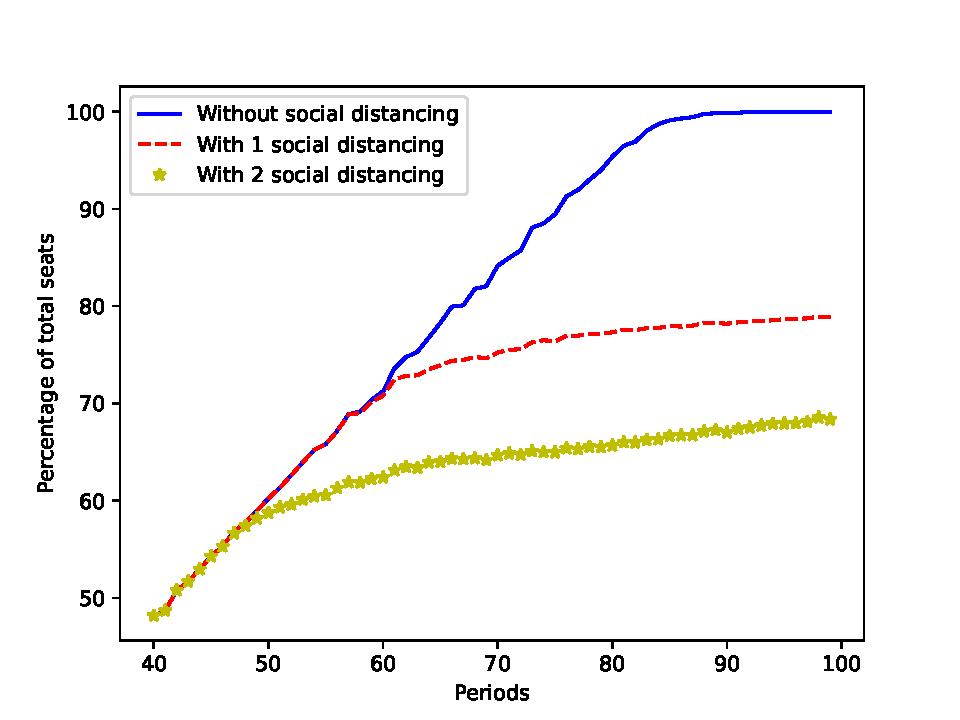
\includegraphics[width=0.8\textwidth]{./Figures/distance.pdf}
  \caption{The occupancy rate over demand for different social distancings}
\end{figure}



We examine the impact of implementing social distancing on the occupancy rate and explore strategies to minimize revenue loss. Consider the situation where the gap point is $\tilde{T}$ and is determined by the parameters $\delta$, $\gamma$, $M$, and $\tilde{L}$. The corresponding occupancy rate is $\Gamma(\tilde{T})$. When the actual number of people (demand) is less than $\tilde{L} \cdot \Gamma(\tilde{T})$, implementing social distancing does not affect the revenue. However, if the actual number of people exceeds $\tilde{L} \cdot \Gamma(\tilde{T})$, enforcing social distancing measures will lead to a reduction in revenue. The extent of this loss can be assessed through simulations by using the specified parameters. To mitigate the potential loss, the seller can increase the value of $\gamma$. This can be achieved by implementing certain measures, such as setting a limit on the number of single-person groups or allowing for larger group sizes. The government can set a requirement for a higher occupancy rate limit, for example, for family movies in cinemas, $\gamma$ will be relatively large, so a higher occupancy rate limit can be set. By doing so, the objective is to minimize the negative impact of social distancing while maximizing revenue within the constraints imposed by the occupancy rate.